\documentclass[]{article}
\usepackage{ctex,hyperref}% 输出汉字
\usepackage{amsmath,amssymb,amsfonts}
\usepackage{amsthm,amsmath,amssymb}
\usepackage{mathrsfs}
%opening
\usepackage{setspace}
\usepackage{lipsum}
\usepackage{graphicx}% 图片插入宏包
\usepackage{subfigure}% 并排子图
\usepackage{float}% 浮动环境,用于调整图片位置
\usepackage[export]{adjustbox}% 防止过宽的图片
\usepackage{amsmath}
\usepackage{extarrows}
\usepackage{arydshln}
\graphicspath{{Figures/}}%文章所用图片在当前目录下的 Figures目录
\usepackage{hyperref} %生成引用链接
\usepackage{cleveref} %实现图片和表格、公式的引用
%%链接设置
\hypersetup{colorlinks = false}
\title{角动量的耦合}
\author{步允霆}

\begin{document}
	
	\maketitle
	\tableofcontents
\section{问题的梗概}
\subsection{态空间}
我们考虑两个粒子的体系,给这两个子体系的各个量分别用指标1和2表示。\par
在子体系(1)的态空间$\mathscr{E}_1$中,我们假设已经知道一个标准基${|k_1,j_1,m_1\rangle}$,他由$\boldsymbol{J}_1^2$和$J_{1z}$的共同本征矢构成,这里的$\boldsymbol{J}_1$是子体系(1)的角动量算符:
\begin{subequations}
	\begin{equation}
		\boldsymbol{J}_1^2|k_1,j_1,m_1\rangle=j_1(j_1+1)\hbar^2|k_1,j_1,m_1\rangle
	\end{equation}
	\begin{equation}
		J_{1z}|k_1,j_1,m_1\rangle=m_1\hbar|k_1,j_1,m_1\rangle 
	\end{equation}
	\begin{equation}
		J_{1\pm}|k_1,j_1,m_1\rangle=\hbar\sqrt{j_1(j_1+1)-m_1(m_1\pm1)}|k_1,j_1,m_1\pm1\rangle
	\end{equation}
\end{subequations}
同样,子体系(2)的态空间$\mathscr{E}_2$和另一个标准基${|k_2,j_2,m_2\rangle}$相联系:
\begin{subequations}
	\begin{equation}
		\boldsymbol{J}_2^2|k_2,j_2,m_2\rangle=j_2(j_2+1)\hbar^2|k_2,j_2,m_2\rangle
	\end{equation}
	\begin{equation}
		J_{2z}|k_2,j_2,m_2\rangle=m_2\hbar|k_2,j_2,m_2\rangle
	\end{equation}
	\begin{equation}
		J_{2\pm}|k_2,j_2,m_2\rangle=\hbar\sqrt{j_2(j_2+1)-m_2(m_2\pm1)}|k_2,j_2,m_2\pm1\rangle
	\end{equation}
\end{subequations}

	总体系的态空间是$\mathscr{E}_1$和$\mathscr{E}_2$的张量积:
\begin{equation}
	\mathscr{E}=\mathscr{E}_1\otimes\mathscr{E}_2
\end{equation}
我们已经知道这个空间中的一个基,他由$\mathscr{E}_1$和$\mathscr{E}_2$中已选定的基的张量积构成,可将这个基中的矢量记作:
\begin{align}
	&|k_1,k_2;j_1,j_2;m_1,m_2\rangle\nonumber\\
	&|k_1,k_2;j_1,j_2;m_1,m_2\rangle=|k_1,j_1,m_1\rangle\otimes|k_2,j_2,m_2\rangle
	\label{c8c8}
\end{align}

我们可将空间看做两两正交的诸子空间$\mathscr{E}(k,j)$的直和,这些空间具有下述性质:\par 
(1)$\mathscr{E}(k,j)$是$(2j+1)$维的。\par 
(2)$\mathscr{E}(k,j)$在$\boldsymbol{J}^2,J_z,J_\pm$的作用下,具有空间不变性,即这些算符只在每一个子空间$\mathscr{E}(k,j)$内才有非零矩阵元。\par 
(3)在一个子空间$\mathscr{E}(k,j)$内,角动量$\boldsymbol{J}$的任意函数$F(\boldsymbol{J})$的矩阵元与$k$无关。

因而,空间$\mathscr{E}$就是得自一个子空间$\mathscr{E}_1(k_1,j_1)$和一个子空间$\mathscr{E}_2(k_2,j_2)$的张量积的子空间$\mathscr{E}(k_1,k_2,j_1,j_2)$的直和:
\begin{equation}
	\mathscr{E}(k_1,k_2,j_1,j_2)=\mathscr{E}_1(k_1,j_1)\otimes\mathscr{E}_2(k_2,j_2)
	\label{c11c11}
\end{equation}
子空间$\mathscr{E}(k_1,k_2,j_1,j_2)$的维数是$(2j_1+1)(2j_2+1)$;他在$\boldsymbol{J}_1$和$\boldsymbol{J}_2$的作用下具有空间不变性。
\subsection{对易关系}
所考虑的体系的总角动量由下式定义:
\begin{equation}
	\boldsymbol{J}=\boldsymbol{J}_1+\boldsymbol{J}_2
\end{equation}
这里$\boldsymbol{J}_1$和$\boldsymbol{J}_2$是在不同的空间$\mathscr{E}_1$和$\mathscr{E}_2$中起作用的算符的延伸,因而是对易的。当然,$\boldsymbol{J}_1$的诸分量,$\boldsymbol{J}_2$的诸分量都满足作为角动量特征的那些对易关系。很容易验证,$\boldsymbol{J}$同样满足那些关系式。\par 
由于$\boldsymbol{J}_1$和$\boldsymbol{J}_2$分别和$\boldsymbol{J}_1^2$与$\boldsymbol{J}_2^2$对易,$\boldsymbol{J}$也就这样;特别的,$\boldsymbol{J}^2$与$J_z$可以和$\boldsymbol{J}_1^2$与$\boldsymbol{J}_2^2$对易:
\begin{subequations}
	\begin{equation}
		[J_z,\boldsymbol{J}_1^2]=[J_z,\boldsymbol{J}_2^2]=0
	\end{equation}
	\begin{equation}
		[\boldsymbol{J}^2,\boldsymbol{J}_1^2]=[\boldsymbol{J}^2,\boldsymbol{J}_2^2]=0
	\end{equation}
	\label{c13c13}
\end{subequations}
另一方面,$J_{1z}$与$J_{2z}$显然可以和$J_z$对易
\begin{equation}
	[J_{1z},J_{z}]=[J_{2z},J_{z}]=0
\end{equation}
但不能和$\boldsymbol{J}^2$对易。实际上,$\boldsymbol{J}^2$可以通过$\boldsymbol{J}_1$与$\boldsymbol{J}_2$来表示:
\begin{equation}
	\boldsymbol{J}^2=\boldsymbol{J}^2_1+\boldsymbol{J}^2_2+2\boldsymbol{J}_1\cdot\boldsymbol{J}_2
\end{equation}
但是,$\boldsymbol{J}^2$既不能与$J_{1z}$也不能与$J_{2z}$对易:
\begin{align}
	[\boldsymbol{J}^2,J_{1z}]&=[\boldsymbol{J}^2_1+\boldsymbol{J}_2^2+2\boldsymbol{J}_1\cdot\boldsymbol{J}_2,J_{1z}]\nonumber\\
	&=2[\boldsymbol{J}_1\cdot\boldsymbol{J}_2,J_{1z}]\nonumber\\
	&=2[J_{1x}J_{2x}+J_{1y}J_{2y},J_{1z}]\nonumber\\
	&=2\mathrm{i}\hbar(-J_{1y}J_{2x}+J_{1x}J_{2y})
\end{align}
我们可以将$\boldsymbol{J}^2$的表示式变换为
\begin{equation}
	\boldsymbol{J}^2=\boldsymbol{J}^2_1+\boldsymbol{J}_2^2+2J_{1z}J_{2z}+J_{1+}J_{2-}+J_{1-}J_{2+}
\end{equation}
这是因为
\begin{align}
	\boldsymbol{J}_1\cdot\boldsymbol{J}_2&=J_{1x}J_{2x}+J_{1y}J_{2y}+J_{1z}J_{2z}\nonumber\\
	&\dfrac{1}{2}(J_{1+}J_{2-}+J_{1-}J_{2+})+J_{1z}J_{2z}
\end{align}
\subsection{有待进行的基的变换}
基\eqref{c8c8}中的一个矢量$|k_1,k_2;j_1,j_2;m_1,m_2\rangle$同时是观察算符:
\begin{equation}
	\boldsymbol{J}_1^2,\boldsymbol{J}_2^2,J_{1z},J_{2z}
\end{equation}
的本征矢,分别对应于本征值$j_1(j_1+1)\hbar^2,j_2(j_2+1)\hbar^2,m_1\hbar,m_2\hbar$.\eqref{c8c8}式中的基适用于研究两个子体系的各自的角动量$\boldsymbol{J}_1$和$\boldsymbol{J}_2$。\par 
根据\eqref{c13c13}式,观察算符
\begin{equation}
	\boldsymbol{J}_1^2,\boldsymbol{J}_2^2,\boldsymbol{J}^2,J_z
\end{equation}
互相对易。我们要构成这些观察算符的共同本征矢的一个正交归一集合;这个新的基将适用于研究体系的总角动量。这个基和前面那个基不是相同的,因为$\boldsymbol{J}^2$不能和$J_{1z}$与$J_{2z}$对易。\par 
由\eqref{c11c11}定义的$\mathscr{E}$的子空间$\mathscr{E}(k_1,k_2;j_1,j_2)$,在$\boldsymbol{J}_1$和$\boldsymbol{J}_2$的一切算符函数的作用下,具有整体不变性,因而在总角动量$\boldsymbol{J}$的一切函数的作用下也具有整体不变性。由此推知,我们想要对角化的观察算符$\boldsymbol{J}^2$和$J_z$,只在同一子空间$\mathscr{E}(k_1,k_2;j_1,j_2)$的诸矢量之间,才有非零矩阵元;在\eqref{c8c8}的基中,表示$\boldsymbol{J}^2$和$J_z$的矩阵是分块对角化的,也就是说,这种矩阵被分解为一系列子矩阵,其中的每一个对应于确定的子空间间$\mathscr{E}(k_1,k_2;j_1,j_2)$。于是,问题归结于每一个子空间间$\mathscr{E}(k_1,k_2;j_1,j_2)$内部的基的变换,这些子空间的维数$(2j_1+1)(2j_2+1)$是有限的。\par 
此外,在\eqref{c8c8}的基中,$\boldsymbol{J}_1$和$\boldsymbol{J}_2$的一个任意函数的矩阵元与$k_1$及$k_2$无关;当然,$\boldsymbol{J}^2$和$J_z$的矩阵元也是这样的。因而$\boldsymbol{J}^2$和$J_z$的对角化问题,在对应于同一个$j_1$和同一个$j_2$的一切子空间$\mathscr{E}(k_1,k_2;j_1,j_2)$中,是完全相同的。正是由于这个原因,我们通常说,将角动量$j_1$和$j_2$相加,而不指名其他量子数。为了书写简便,我们省略$k_1$和$k_2$,用$\mathscr{E}(j_1,j_2)$表示子空间$\mathscr{E}(k_1,k_2;j_1,j_2)$,用$|j_1,j_2;m_1,m_2\rangle$表示在\eqref{c8c8}的基中属于这个子空间的诸矢量:
\begin{subequations}
	\begin{equation}
		\mathscr{E}(j_1,j_2)\equiv\mathscr{E}(k_1,k_2;j_1,j_2)
	\end{equation}
	\begin{equation}
		|j_1,j_2;m_1,m_2\rangle\equiv|k_1,k_2;j_1,j_2;m_1,m_2\rangle
		\label{c21bc21b}
	\end{equation}
\end{subequations}

而$\mathscr{E}(j_1,j_2)$是两两正交的诸子空间$\mathscr{E}(k,j)$的直和,其中的每一个在算符$\boldsymbol{J}^2,J_z,J_+,J_-$的作用下是具有整体不变性:
\begin{equation}
	\mathscr{E}(j_1,j_2)=\sum\limits_{\oplus}\mathscr{E}(k,j)
	\label{c22c22}
\end{equation}
归结起来,我们要解决的是两方面的问题:\par 
(1)假设已知$j_1$和$j_2$,问公式\eqref{c22c22}中的$J$的值如何?与每一个值相联系的不同的子空间$\mathscr{E}(k,j)$有多少个?\par 
(2)怎样将$\boldsymbol{J}^2$和$J_z$的属于子空间$\mathscr{E}(j_1,j_2)$的本征矢在基${|j_1,j_2;m_1,m_2\rangle}$中展开?
\section{$\boldsymbol{J}^2$和$J_z$的本征值}
\subsection{两个自旋1/2的耦合的特例}
\subsubsection{态空间}
我们将一个正交归一基,即${|\varepsilon_1,\varepsilon_2\rangle}$,具体的写出来,这就是:
\begin{equation}
	\{|\varepsilon_1,\varepsilon_2\rangle\}=\{|+,+\rangle,|+,-\rangle,|-,+\rangle,|-,-\rangle\}
	\label{b1b1}
\end{equation}
这些矢量是观察算符$\boldsymbol{S}_1^2,S_{1z},\boldsymbol{S}_2^2,S_{2z}$的本征矢:
\begin{subequations}
	\begin{equation}
		\boldsymbol{S}_1^2|\varepsilon_1,\varepsilon_2\rangle=\boldsymbol{S}_2^2|\varepsilon_1,\varepsilon_2\rangle=\dfrac{3}{4}\hbar^2|\varepsilon_1,\varepsilon_2\rangle
	\end{equation}
	\begin{equation}
		S_{1z}|\varepsilon_1,\varepsilon_2\rangle=\varepsilon_1\dfrac{\hbar}{2}|\varepsilon_1,\varepsilon_2\rangle
		\label{b2bb2b}
	\end{equation}
	\begin{equation}
		S_{2z}|\varepsilon_1,\varepsilon_2\rangle=\varepsilon_2\dfrac{\hbar}{2}|\varepsilon_1,\varepsilon_2\rangle
		\label{b2cb2c}
	\end{equation}
\end{subequations}
$\boldsymbol{S}_1^2,S_{1z},\boldsymbol{S}_2^2,S_{2z}$构成一个CSCO。
\subsubsection{对易关系}
我们将体系的总自旋定义为:
\begin{equation}
	\boldsymbol{S}=\boldsymbol{S}_1+\boldsymbol{S}_2
\end{equation}

由于$\boldsymbol{S}_1\cdot\boldsymbol{S}_2$可以对易,我们便可以得到算符$\boldsymbol{S}^2$:
\begin{equation}
	\boldsymbol{S}^2=(\boldsymbol{S}_1+\boldsymbol{S}_2)^2=\boldsymbol{S}_1^2+\boldsymbol{S}_2^2+2\boldsymbol{S}_1\cdot\boldsymbol{S}_2
\end{equation}
标量积$\boldsymbol{S}_1\cdot\boldsymbol{S}_2$可以通过算符$S_{1\pm},S_{1z}$和$S_{2\pm},S_{2z}$来表示,实际上,很容易证明:
\begin{align}
	\boldsymbol{S}_1\cdot\boldsymbol{S}_2&=S_{1x}S_{2x}+S_{1y}S_{2y}+S_{1z}S_{2z}\nonumber\\
	&=\dfrac{1}{2}(S_{1+}S_{2-}+S_{1-}S_{2+})+S_{1z}S_{2z}
\end{align}

注意,由于$\boldsymbol{S}_1$和$\boldsymbol{S}_2$分别于$\boldsymbol{S}_1^2$及$\boldsymbol{S}_2^2$对易,故$\boldsymbol{S}$的三个分量也具有这样的性质;特别的,$\boldsymbol{S}^2$和$S_z$可以与$\boldsymbol{S}_1^2$及$\boldsymbol{S}_2^2$对易:
\begin{subequations}
	\begin{equation}
		[S_z,\boldsymbol{S}_1^2]=[S_z,\boldsymbol{S}_2^2]=0
	\end{equation}
	\begin{equation}
		[\boldsymbol{S}^2,\boldsymbol{S}_1^2]=[\boldsymbol{S}^2,\boldsymbol{S}_2^2]=0
	\end{equation}
\end{subequations}
此外,$S_z$显然与$S_{1z}$及$S_{2z}$对易:
\begin{equation}
	[S_z,S_{1z}]=[S_z,S_{2z}]=0
\end{equation}
但是,$\boldsymbol{S}^2$既不能与$S_{1z}$也不能与$S_{2z}$对易:
\begin{align}
	[\boldsymbol{S}^2,S_{1z}]&=[\boldsymbol{S}_1^2+\boldsymbol{S}_2^2+2\boldsymbol{S}_1\cdot\boldsymbol{S}_2,S_{1z}]\nonumber\\
	&=2[\boldsymbol{S}_1\cdot\boldsymbol{S}_2,S_{1z}]\nonumber\\
	&=2[S_{1x}S_{2x}+S_{1y}S_{2y},S_{1z}]\nonumber\\
	&=2\mathrm{i}\hbar(-S_{1y}S_{2x}+S_{1x}S_{2y})
\end{align}
当然,$\boldsymbol{S}^2$和$S_{2z}$的对易子正好和上式反号,所以,$S_z=S_{1z}+S_{2z}$和$\boldsymbol{S}^2$对易。
\subsubsection{有待进行的基的变换}
我们已经看过,\eqref{b1b1}式中的基是由下列CSCO:
\begin{equation}
	\{\boldsymbol{S}^2_1,\boldsymbol{S}^2_2,S_{1z},S_{2z}\}
\end{equation}
的共同本征矢构成的。此外,我们刚才证明过下列四个观察算符:
\begin{equation}
	\boldsymbol{S}^2_1,\boldsymbol{S}^2_2,\boldsymbol{S}^2,S_z
	\label{b11b11}
\end{equation}
互相对易,他们也构成一个CSCO。\par 
要将两个自旋$\boldsymbol{S}_1$和$\boldsymbol{S}_2$相加,就是要构成算符集合\eqref{b11b11}的共同本征矢的一个正交归一集合。因$\boldsymbol{S}^2$不能和$S_{1z}$及$S_{2z}$对易,故这个集合将不同于\eqref{b1b1}中的集合。我们将这个新的基矢量记作$|S,M\rangle$,而$\boldsymbol{S}^2_1$和$\boldsymbol{S}^2_2$的本征值的符号略去不写。于是,矢量$|S,M\rangle$满足下列方程:
\begin{subequations}
	\begin{equation}
		\boldsymbol{S}^2_1|S,M\rangle=\boldsymbol{S}^2_2|S,M\rangle=\dfrac{3}{4}\hbar^2|S,M\rangle
		\label{b12ab12a}
	\end{equation}
	\begin{equation}
		\boldsymbol{S}^2|S,M\rangle=S(S+1)\hbar^2|S,M\rangle
	\end{equation}
	\begin{equation}
		S_z|S,M\rangle=M\hbar|S,M\rangle
	\end{equation}
\end{subequations}
由于$\boldsymbol{S}$是一个角动量,因此,$S$只能是正的整数或半整数,而$M$的值则在$-S$与$+S$之间变化,每次改变一个单位。
\subsubsection{$S_z$的本征值及其简并度}
对于$\boldsymbol{S}^2_1$与$\boldsymbol{S}^2_2$这两个算符,态空间的所有矢量都是他们的本征矢,而且属于同一本征值$3\hbar^2/4$,所以,无论$|S,M\rangle$为任何右矢,\eqref{b12ab12a}都会自动满足。\par 
由于$S_z$可以和CSCO中四个观察算符对易,因此,我们可以预料,基$\{|\varepsilon_1,\varepsilon_2\rangle\}$中的矢量本来就是$S_z$的本征矢。我们可以用\eqref{b2bb2b}\eqref{b2cb2c}实际检验一下:
\begin{equation}
	S_z|\varepsilon_1,\varepsilon_2\rangle=(S_{1z}+S_{2z})|\varepsilon_1,\varepsilon_2\rangle=\dfrac{1}{2}(\varepsilon_1+\varepsilon_2)|\varepsilon_1,\varepsilon_2\rangle
\end{equation}
由此可见,$|\varepsilon_1,\varepsilon_2\rangle$是$S_z$的本征矢,属于本征值:
\begin{equation}
	M=\dfrac{1}{2}(\varepsilon_1+\varepsilon_2)
\end{equation}
由于$\varepsilon_1$和$\varepsilon_2$中的每一个都可以等于$\pm1$,从而推知$M$可取的值为$+1,0,-1$。\par 
$M=1$和$M=-1$这两个值是非简并的,因为对应于前者的本征矢只有$|+,+\rangle$,对应于后者的只有$|-,-\rangle$。反之,$M=0$是二重简并的,因为有两个正交的本征矢$|+,-\rangle$和$|-,+\rangle$与之相联系;这两个矢量的一切线性组合都是$S_z$的本征矢,属于本征值$0$。\par 
从基$\{|\varepsilon_1,\varepsilon_2\rangle\}$中表示$S_z$的矩阵来看,这个结果是很明显的;如果我们按\eqref{b1b1}中的顺序来安排基矢量,那么这个矩阵可以写作:
\begin{equation}
	(S_z)=\hbar\begin{pmatrix}
		1&0&0&0\\
		0&0&0&0\\
		0&0&0&0\\
		0&0&0&-1\\
	\end{pmatrix}
\end{equation}

现在,剩下的任务仅仅是计算在基$\{|\varepsilon_1,\varepsilon_2\rangle\}$中表示$\boldsymbol{S}^2$的矩阵,再将他对角化。事先,我们就知道这个矩阵并不是对角化的,因为$\boldsymbol{S}^2$不能与$S_{1z}$及$S_{2z}$对易。
\subsubsection{表示$\boldsymbol{S}^2$矩阵的计算}
我们把算符$\boldsymbol{S}^2$作用于每一个基矢量,为此:
\begin{equation}
	\boldsymbol{S}^2=\boldsymbol{S}_1^2+\boldsymbol{S}_2^2+2S_{1z}S_{2z}+S_{1+}S_{2-}+S_{1-}S_{2+}
\end{equation}
四个矢量$|\varepsilon_1,\varepsilon_2\rangle$都是$\boldsymbol{S}_1^2,\boldsymbol{S}_2^2,S_{1z},S_{2z}$的本征矢,而算符$S_{1\pm}$和$S_{2\pm}$的作用也可以用角动量升降算符导出,这样,我们得到:
\begin{subequations}
	\begin{align}
		\boldsymbol{S}^2|+,+\rangle&=\left( \dfrac{3}{4}\hbar^2+\dfrac{3}{4}\hbar^2\right) |+,+\rangle+\dfrac{1}{2}\hbar^2|+,+\rangle\nonumber\\
		&=2\hbar^2|+,+\rangle
	\end{align}
	\begin{align}
		\boldsymbol{S}^2|+,-\rangle&=\left( \dfrac{3}{4}\hbar^2+\dfrac{3}{4}\hbar^2\right) |+,-\rangle-\dfrac{1}{2}\hbar^2|+,-\rangle+\hbar^2|-,+\rangle\nonumber\\
		&=\hbar^2[|+,-\rangle+|-,+\rangle]
	\end{align}	
		\begin{align}
		\boldsymbol{S}^2|-,+\rangle&=\left( \dfrac{3}{4}\hbar^2+\dfrac{3}{4}\hbar^2\right) |-,+\rangle-\dfrac{1}{2}\hbar^2|-,+\rangle+\hbar^2|+,-\rangle\nonumber\\
		&=\hbar^2[|-,+\rangle+|+,-\rangle]
	\end{align}	
	\begin{align}
		\boldsymbol{S}^2|-,-\rangle&=\left( \dfrac{3}{4}\hbar^2+\dfrac{3}{4}\hbar^2\right) |-,-\rangle+\dfrac{1}{2}\hbar^2|-,-\rangle\nonumber\\
		&=2\hbar^2|-,-\rangle
	\end{align}
\end{subequations}

于是,在四个矢量$|\varepsilon_1,\varepsilon_2\rangle$组成的基中,表示$\boldsymbol{S}^2$的矩阵可以写成:
\begin{equation}
	(\boldsymbol{S}^2)=\hbar^2\begin{pmatrix}
		2&0&0&0\\
		0&1&1&0\\
		0&1&1&0\\
		0&0&0&2\\
	\end{pmatrix}
	\label{b18b18}
\end{equation}
\subsubsection{$\boldsymbol{S}^2$的本征值和本征矢}
矩阵\eqref{b18b18}可以分为三个子矩阵,其中的两个是一阶的,这就是说,$|+,+\rangle$和$|-,-\rangle$都是$\boldsymbol{S}^2$的本征矢,他们对应的两个本征值都等于$2\hbar^2$。\par 
现在还要将子矩阵:
\begin{equation}
	(\boldsymbol{S}^2)_0=\hbar^2\begin{pmatrix}
		1&1\\
		1&1\\
	\end{pmatrix}
	\label{b19b19}
\end{equation}
对角化。这个子矩阵在$|+,-\rangle$和$|-,+\rangle$所张成的二维子空间(即$S_z$的对应于$M=0$的本征子空间)内部表示$\boldsymbol{S}^2$。矩阵\eqref{b19b19}的本征值$\lambda\hbar^2$可以得自下列特征方程:
\begin{equation}
	(1-\lambda)^2-1=0
\end{equation}
的解。此方程的跟$\lambda=0$和$\lambda=2$,他们给出了$\boldsymbol{S}^2$的另外两个本征值:$0,2\hbar^2$,以及他们的本征值:
\begin{subequations}
	\begin{equation}
		\dfrac{1}{\sqrt{2}}[|+,-\rangle+|-,+\rangle]\quad\text{对应于本征值$2\hbar^2$}
		\label{b21ab21a}
	\end{equation}
	\begin{equation}
		\dfrac{1}{\sqrt{2}}[|+,-\rangle-|-,+\rangle]\quad\text{对应于本征值$0$}
		\label{b21bb21b}
	\end{equation}
\end{subequations}

可见算符$\boldsymbol{S}^2$有两个不同的本征值:$0,2\hbar^2$。第一个是非简并的,和他对应的矢量是\eqref{b21bb21b};第二个本征值是三重简并的,在与他相联系的本征子空间中,矢量$|+,-\rangle,|-,-\rangle$,和\eqref{b21ab21a}构成一个正交归一基。\par 
于是,四维空间$\mathscr{E}(1/2,1/2)$分解为与$S=1$相联系的一个子空间(三维的)以及与$S=0$相联系的一个子空间(一维的)。
\subsection{$J_z$的本征值及其简并度}
我们将在$(2j_1+1)(2j_2+1)$维的一个确定的子空间$\mathscr{E}(j_1,j_2)$的内部来分析问题。下面假设$j_1$和$j_2$的相对大小符合不等式:
\begin{equation}
	j_1\geqslant j_2
\end{equation}

诸矢量$|j_1,j_2;m_1,m_2\rangle$本来就是$J_z$的本征矢:
\begin{align}
	J_z|j_1,j_2;m_1,m_2\rangle&=(J_{1z}+J_{2z})|j_1,j_2;m_1,m_2\rangle\nonumber\\
	&=(m_1+m_2)\hbar|j_1,j_2;m_1,m_2\rangle
\end{align}
对应的本征值$M\hbar$应该取这样的值,使得
\begin{equation}
	M=m_1+m_2
\end{equation}
因而,$M$应取下列的数值:
\begin{equation}
	j_1+j_2,j_1+j_2-1,j_1+j_2-2,\cdots,-(j_1+j_2)
	\label{c26c26}
\end{equation}

为了求得这些数值的简并度$g_{j_1,j_2}(M)$,我们可以采用下述的几何方法。对于每一个矢量$|j_1,j_2;m_1,m_2\rangle$,我们用平面上的一个点来和他对应,点的横坐标为$m_1$,纵坐标为$m_2$。所有这些都落在一个矩形的内部或其边缘上,这个矩阵的顶点的坐标是:$(j_1,j_2),(j_1,-j_2),(-j_1,-j_2)$和$(-j_1,j_2)$。例如,取$j_1=2,j_2=1$;那么,对应于基矢量的15个点的位置如图1。对应于$M=m_1+m_2$的同一个值的诸点都在平行于第二角平分线的同一条直线上;因而,这些点的个数就是那个$M$值的简并度$g_{j_1,j_2}(M)$。\par 
\begin{figure}[H]
	\centering
	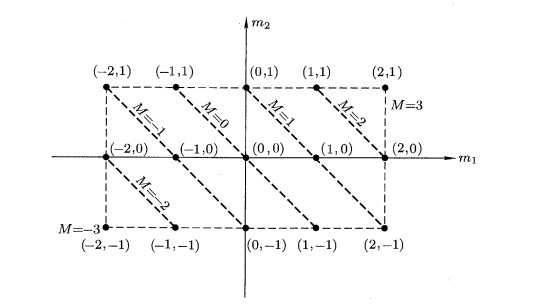
\includegraphics[scale=0.6]{1.png}
	\caption{对于右矢$|j_1,j_2;m_1,m_2\rangle$而言,$(m_1,m_2)$的可能值组}
	\label{Figure 1}
\end{figure}

下面再来考察$M$的各个值,并做出每个值确定的平行于第二角平分线的诸直线;$M=j_1+j_2$是简并的,因为他所确定的直线仅仅通过矩阵的右上顶角$(j_1,j_2)$,即:
\begin{equation}
	g_{j_1,j_2}(j_1+j_2)=1
	\label{c27c27}
\end{equation}
$M=j_1+j_2-1$是二重简并的,因为对应的直线通过点$(j_1,j_2-1)$和点$(j_1-1,j_2)$,即:
\begin{equation}
	g_{j_1,j_2}(j+1+j_2-1)=2
	\label{c28c28}
\end{equation}
像这样,$M$的值每减小一个单位,简并度就增加一个单位,这个过程一直进行到矩阵的右下顶点$(m_1=j_1,m_2=-j_2)$即直到$M=j_1-j_2$;于是这条直线上的点的个数达到极大值,即:
\begin{equation}
	g_{j_1,j_2}(j+1-j_2)=2j_2+1
\end{equation}
如果$M$的值捡到小于$j_1-j_2$,则$g_{j_1,j_2}(M)$首先保持其极大值不变,一直保持到与$M$对应的直线以矩阵的整个宽度与之相割,即一直保持到该直线通过矩形的左上顶点$(m_1=-j_1,m_2=j_2)$;这时:
\begin{equation}
	g_{j_1,j_2}(M)=2j_2+1,\quad for \  -(j_1-j_2)\leqslant M\leqslant j_1-j_2
	\label{c30c30}
\end{equation}
最后,若$M$的值小于$-(j_1-j_2)$,则对应的直线不能再与矩阵的水平上边相交,于是,$M$的值减小一个单位,$g_{j_1,j_2}(M)$的值也减小一个单位,以致$M=-(j_1+j_2)$时,简并度重新回到了1;因而
\begin{equation}
	g_{j_1,j_2}(-M)=g_{j_1,j_2}(M)
\end{equation}
对于$j_1=2,j_2=1$的情况,全部归结于图2,此图描绘了$g_{2,1}(M)$随$M$变化的情况。
\begin{figure}[H]
	\centering
	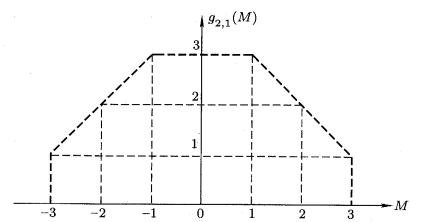
\includegraphics[scale=0.6]{2.png}
	\caption{$g_{2,1}(M)$随$M$变化的情况}
	\label{Figure 2}
\end{figure}
\subsection{$\boldsymbol{J}^2$的本征值}
首先我们注意列举$M$的值的\eqref{c26c26},如果$j_1$和$j_2$都是整数或都是半整数,则$M$的值都是整数;如果$j_1$和$j_2$中,一个是整数,一个是半整数,则$M$的值都是半整数。因而$J$的对应数值,在前一种情况下也将都是整数,而在后一种情况下,也将都是半整数。\par 
由于$M$所达到的极大值为$j_1+j_2$,故$J$的每一个大于$j_1+j_2$的值在空间$\mathscr{E}(j_1,j_2)$中都不能实现,于是也不会出现在直和\eqref{c22c22}中。与$J=j_1+j_2$联系着一个不变子空间(因为$M=j_1+j_2$这个值存在),而且只联系着这样一个(因为$M=j_1+j_2$是非简并的)。在这个子空间$\mathscr{E}(J=j_1+j_2)$中,有一个而且只有一个矢量,他所对应的$M=j_1+j_2-1$但$M$的这个值在空间$\mathscr{E}(j_1,j_2)$中是二重简并的;于是$J=j_1+j_2-1$也是可以实现的,而且与他对应着一个唯一的不变子空间$\mathscr{E}(J=j_1+j_2-1)$。\par 
更普遍一点,我们用$p_{j_1,j_2}(J)$表示空间$\mathscr{E}(j_1,j_2)$中与$J$的一个给定值相联系的子空间$\mathscr{E}(k,J)$的数目;也就是对于$J$的这个值,$k$的互异值的个数;这个$p_{j_1,j_2}(J)$与$g_{j_1,j_2}(M)$之间有一个简单的关系。实际上,我们来考虑$M$的一个特殊值;在符合$J\geqslant|M|$的每一个子空间$\mathscr{E}(k,J)$中,都有一个而且只有一个矢量与$M$的那个值对应,于是那个值在空间$\mathscr{E}(j_1,j_2)$中的简并度$g_{j_1,j_2}(M)$可以写作:
\begin{align}
	g_{j_1,j_2}(M)=&p_{j_1,j_2}(J=|M|)+p_{j_1,j_2}(J=|M|+1)\nonumber\\
	&p_{j_1,j_2}(J=|M|+2)+\cdots 
\end{align}
由此式,可以反过来用$g_{j_1,j_2}(M)$来表示$p_{j_1,j_2}(J)$:
\begin{align}
	p_{j_1,j_2}(J)&=g_{j_1,j_2}(M=J)-g_{j_1,j_2}(M=J-1)\nonumber\\
	&=g_{j_1,j_2}(M=-J)-g_{j_1,j_2}(M=-J-1)
\end{align}

于是,上一节的结果可以用来直接确定合空间$\mathscr{E}(j_1,j_2)$中量子数$J$实际可取的那些值以及与他们相联系的不变子空间$\mathscr{E}(k,J)$的数目。首先,我们显然有:
\begin{equation}
	p_{j_1,j_2}(J)=0,\quad for \  J>j_1+j_2
\end{equation}
这是因为对于$|M|>j_1+j_2,g_{j_1,j_2}(M)$为零。此外,根据\eqref{c27c27}\eqref{c28c28},有:
\begin{subequations}
	\begin{equation}
		p_{j_1,j_2}(J=j_1+j_2)=g_{j_1,j_2}(M=j_1+j_2)=1
	\end{equation}
	\begin{equation}
		p_{j_1,j_2}(J=j_1+j_2-1)=g_{j_1,j_2}(M=j_1+j_2-1)-g_{j_1,j_2}(M=j_1+j_2)=1
	\end{equation}
\end{subequations}
这样,我们可以逐个地求得$p_{j_1,j_2}(J)$的全体数值
\begin{subequations}
	\begin{equation}
		p_{j_1,j_2}(J=j_1+j_2-2)=1,\cdots,
	\end{equation}
	\begin{equation}
		\cdots,p_{j_1,j_2}(J=j_1-j_2)=1
	\end{equation}
\end{subequations}
最后,根据\eqref{c30c30},有:
\begin{equation}
	p_{j_1,j_2}(J)=0,\quad for \  J<j_1-j_2
\end{equation}

对于$j_1$和$j_2$的固定值,$\boldsymbol{J}^2$的本征值中的$J$应为:
\begin{equation}
	J=j_1+j_2,j_1+j_2-1,j_1+j_2-2,\cdots,|j_1-j_2|
	\label{c38c38}
\end{equation}
与每一个这样的值联系着唯一的一个不变子空间$\mathscr{E}(J)$,于是,\eqref{c22c22}中的指标$k$实际上没有用了。特别地,由此推知,如果在\eqref{c38c38}的集合中,取定$J$的一个值,随之取定与他相容的一个$M$的值,那么,在空间$\mathscr{E}(j_1,j_2)$中,与他们对应的矢量只有一个;实际上,$J$的数值就足以确定子空间$\mathscr{E}(J)$,在这个子空间中,$M$的数值就确定了一个唯一的矢量。换句话说,$\boldsymbol{J}^2$和$J_z$构成$\mathscr{E}(j_1,j_2)$空间中的一个CSCO。\par 
我们可以证明,在空间$\mathscr{E}(j_1,j_2)$中可以实现的$(J,M)$值的组数正好等于该空间维数$(2j_1+1)(2j_2+1)$。实际上,这个数等于:
\begin{equation}
	\sum\limits_{J=j_1-j_2}^{j_1+j_2}(2J+1)
\end{equation}
如果令
\begin{equation}
	J=j_1-j_2+i
\end{equation}
那么,我们可以算出
\begin{align}
	\sum\limits_{J=j_1-j_2}^{j_1+j_2}(2J+1)&=\sum\limits_{i=0}^{2j_2}[2(j_1-j_2+i)+1]\nonumber\\
	&=[2(j_1-j_2)+1](2j_2+1)+2\dfrac{2j_2(2j_2+1)}{2}\nonumber\\
	&=(2j_2+1)(2j_1+1)
\end{align}
\section{$\boldsymbol{J}^2$和$J_z$的共同本征矢}
我们将$\boldsymbol{J}^2$和$J_z$的属于空间$\mathscr{E}(j_1,j_2)$的共同本征矢记作$|J,M\rangle$。严格的说,本来应该在这个记号中注明$j_1$和$j_2$的值,但我们没有注明,因为他们的值和矢量\eqref{c21bc21b}中的相同,而$|J,M\rangle$不过是那些矢量的线性组合。当然,指标$J$和$M$的值与$\boldsymbol{J}^2$和$J_z$的本征值相联系:
\begin{subequations}
	\begin{equation}
		\boldsymbol{J}^2|J,M\rangle=J(J+1)\hbar^2|J,M\rangle
	\end{equation}
	\begin{equation}
		J_z|J,M\rangle=M\hbar|J,M\rangle 
	\end{equation}
\end{subequations}
而矢量$|J,M\rangle$,正如空间$\mathscr{E}(j_1,j_2)$中所有的这些矢量一样,都是$\boldsymbol{J}^2_1$和$\boldsymbol{J}^2_2$的本征矢,分别属于本征值$j_1(j_1+1)\hbar^2$和$j_2(j_2+1)\hbar^2$。
\subsection{两个自旋1/2的特例}
\subsubsection{子空间$\mathscr{E}(S=1)$}
在态空间$\mathscr{E}=\mathscr{E}(1/2,1/2)$中,右矢$|+,+\rangle$是$S_z$的对应于$M=1$的唯一的一个本征矢。由于$\boldsymbol{S}^2$和$S_z$对易,而且$M=1$这个值是非简并的,故右矢$|+,+\rangle$一定也是$\boldsymbol{S}^2$的本征矢。根据之前的分析,$S$的值只能等于1;因此,我们可以如此选择矢量$|S=1,M=1\rangle$的相位,使得:
\begin{equation}
	|1,1\rangle=|+,+\rangle
	\label{c43c43}
\end{equation}

然后,三重态中的其他态就好求了。实际上,根据角动量理论的普遍理论,我们知道:
\begin{align}
	S_-|1,1\rangle&=\hbar\sqrt{1(1+1)-1(1-1)}|1,0\rangle\nonumber\\
	&=\hbar\sqrt{2}|1,0\rangle
\end{align}
因此
\begin{equation}
	|1,0\rangle=\dfrac{1}{\hbar\sqrt{2}}S_-|+,+\rangle
	\label{c45c45}
\end{equation}
于是,可以求得
\begin{align}
	|1,0\rangle&=\dfrac{1}{\hbar\sqrt{2}}(S_{1-}+S_{2-})|+,+\rangle\nonumber\\
	&=\dfrac{1}{\hbar\sqrt{2}}[\hbar|-,+\rangle+\hbar|+,-\rangle]\nonumber\\
	&=\dfrac{1}{\sqrt{2}}[|-,+\rangle+|+,-\rangle]
	\label{c47c47}
\end{align}
最后,我们可以再将算符$S_-$应用于$|1,0\rangle$,也就是将算符$(S_{1-}+S_{2-})$应用于\eqref{c47c47}。这样便得到
\begin{align}
	|1,-1\rangle&=\dfrac{1}{\hbar\sqrt{2}}S_-|1,0\rangle\nonumber\\
	&=\dfrac{1}{\hbar\sqrt{2}}(S_{1-}+S_{2-})\dfrac{1}{\sqrt{2}}[|-,+\rangle+|+,-\rangle]\nonumber\\
	&=\dfrac{1}{2\hbar}[\hbar|-,-\rangle+\hbar|-,-\rangle]\nonumber\\
	&=|-,-\rangle
\end{align}
当然,仿照上面对右矢$|+,+\rangle$所作的推理,本来也可以直接得到最后这个结果。但是,上面这个算法有一点方便之处:这个方法可以确定由于在\eqref{c43c43}中已经给右矢$|+,+\rangle$选定了相位而可能出现在右矢$|1,0\rangle$和$|1,-1\rangle$中的那些相位因子。
\subsubsection{态$|S=0,M=0\rangle$}
子空间$\mathscr{E}(S=0)$中独一无二的矢量$|S=0,M=0\rangle$必须与刚才求得的三个矢量$|1,M\rangle$正交,根据这个简单的条件就可以确定这个矢量。\par 
实际上,矢量$|0,0\rangle$既然正交于$|1,1\rangle=|+,+\rangle$和$|1,-1\rangle=|-,-\rangle$,那么,他只可能是$|+,-\rangle$和$|-,+\rangle$的线性组合:
\begin{equation}
	|0,0\rangle=\alpha|+,-\rangle+\beta|-,+\rangle
\end{equation}
为将他归一化,须使
\begin{equation}
	\langle0,0|0,0\rangle=|\alpha|^2+|\beta|^2=1
	\label{c50c50}
\end{equation}
他与右矢$|1,0\rangle$的标量积等于零,即应有:
\begin{equation}
	\dfrac{1}{\sqrt{2}}(\alpha+\beta)=0
\end{equation}
因此,系数$\alpha$和$\beta$的符号相反,这个条件,并结合\eqref{c50c50},便可确定(除相位因子外):
\begin{equation}
	\alpha=-\beta=\dfrac{1}{\sqrt{2}}\mathrm{e}^{\mathrm{i}\chi}
\end{equation}
式中的$\chi$为任意实数,我们不妨选择$\chi=0$,这样便得到:
\begin{equation}
	|0,0\rangle=\dfrac{1}{\sqrt{2}}[|+,-\rangle-|-,+\rangle]
\end{equation}

至此,我们已经求得四个矢量$|S,M\rangle$,而并不需要在基$\{|\varepsilon_1,\varepsilon_2\}$中表示$\boldsymbol{S}^2$的矩阵的显式。
\subsection{$j_1$和$j_2$是任意的一般情况}
我们已经证明过,$\mathscr{E}(j_1,j_2)$作为不变子空间$\mathscr{E}(J)$的直和的分解式为:
\begin{equation}
	\mathscr{E}(j_1,j_2)=\mathscr{E}(j_1+j_2)\oplus\mathscr{E}(j_1+j_2-1)\oplus\cdots\oplus\mathscr{E}(|j_1-j_2|)
	\label{c54c54}
\end{equation}
下面我们将说明怎样确定张成这些子空间的诸矢量$|J,M\rangle$。
\subsubsection{子空间$\mathscr{E}(J=j_1+j_2)$}
在空间$\mathscr{E}(j_1,j_2)$中,右矢$|j_1,j_2;m_1=j_1,m_2=j_2\rangle$是$J_z$的对应于$M=j_1+j_2$的唯一的一个本征矢。由于$\boldsymbol{J}^2$和$J_z$对易,而且$M=j_1+j_2$这个值是非简并的,故矢量矢$|j_1,j_2;m_1=j_1,m_2=j_2\rangle$一定也是$\boldsymbol{J}^2$的本征矢。根据\eqref{c45c45},$J$的对应值只可能是$j_1+j_2$。我们可以如此选择矢量:
\begin{equation}
	|J=j_1+j_2,M=j_1+j_2\rangle
\end{equation}
的相位,使得:
\begin{equation}
	|j_1+j_2,j_1+j_2\rangle=|j_1,j_2;j_1,j_2\rangle
\end{equation}

根据这个公式,重复应用算符$J_-$,就可以求得符合$J=j_1+j_2$的全体矢量$|J,M\rangle$。于是,根据角动量的普遍公式,有:
\begin{equation}
	J_-|j_1+j_2,j_1+j_2\rangle=\hbar\sqrt{2(j_1+j_2)}|j_1+j_2,j_1+j_2-1\rangle
\end{equation}
现将算符$J_-=J_{1-}+J_{2-}$应用于$|j_1,j_2;j_1,j_2\rangle$,我们便可以求得对应于$J=j_1+j_2$和$M=j_1+j_2-1$的矢量:
\begin{align}
	|j_1+j_2,j_1+j_2-1\rangle&=\dfrac{1}{\hbar\sqrt{2(j_1+j_2)}}J_-|j_1+j_2,j_1+j_2\rangle\nonumber\\
	&=\dfrac{1}{\hbar\sqrt{2(j_1+j_2)}}(J_{1-}+J_{2-})|j_1,j_2;j_1,j_2\rangle\nonumber\\
	&=\dfrac{1}{\hbar\sqrt{2(j_1+j_2)}}[\hbar\sqrt{2j_1}|j_1,j_2;j_1-1,j_2\rangle]\nonumber\\
	&\quad+\hbar\sqrt{2j_2}|j_1,j_2;j_1,j_2-1\rangle]
\end{align}
也就是说
\begin{align}
	|j_1+j_2,j_1+j_2-1\rangle=&\sqrt{\dfrac{j_1}{j_1+j_2}}|j_1,j_2;j_1-1,j_2\rangle\nonumber\\
	&+\sqrt{\dfrac{j_2}{j_1+j_2}}|j_1,j_2;j_1,j_2-1\rangle
	\label{c58c58}
\end{align}
注意,按这种方式,我们求得了对应于$M=j_1+j_2-1$的两个基矢量的线性组合,而且这种组合本身已经是归一化的。\par 
然后,我们重复下面的步骤:将算符$J_-$作用于\eqref{c58c58}两端(在右端,将此算符写作$J_{1-}+J_{2-}$的形式),以构成矢量$|j_1+j_2,j_1+j_2-2\rangle$,像这个逐步进行下去,直到矢量$|j_1+j_2,-(j_1+j_2)\rangle$,我们将会看到他等于矢量$|j_1,j_2;-j_1,-j_2\rangle$。\par 
这样一来,我们便能算出基$\{|J,M\rangle\}$中的前$[2(j_1+j_2)+1]$个矢量,他们对应于$J=j_1+j_2$和$M=j_1+j_2,j_1+j_2-1,\cdots,-(j_1+j_2)$,并张成空间$\mathscr{E}(j_1,j_2)$中的子空间$\mathscr{E}(J=j_1+j_2)$。
\subsubsection{其他子空间$\mathscr{E}(J)$}
现在我们来考虑在空间$\mathscr{E}(j_1,j_2)$中和$\mathscr{E}(j_1+j_2)$互补的空间$\mathscr{J}(j_1+j_2)$。根据\eqref{c54c54},空间$\mathscr{J}(j_1+j_2)$分解为:
\begin{equation}
	\mathscr{J}(j_1,j_2)=\mathscr{E}(j_1+j_2-1)\oplus\mathscr{E}(j_1+j_2-2)\oplus\cdots\oplus\mathscr{E}(|j_1-j_2|)
\end{equation}

在空间$\mathscr{J}(j_1+j_2)$中,$M$的一个给定值的简并度$g^\prime_{j_1,j_2}(M)$比$g_{j_1,j_2}(M)$小1,这是因为空间$\mathscr{E}(j_1+j_2)$仅仅包含与$M$的这个值相联系的一个矢量:
\begin{equation}
	g^\prime_{j_1,j_2}(M)=g_{j_1,j_2}(M)-1
\end{equation}
这一点特别表明,$M=j_1+j_2$这个值在空间$\mathscr{J}(j_1+j_2)$中不复存在,而且新的极大值$M=j_1+j_2-1$是非简并的。如同前一节所述,由此可以推知,对应的矢量一定正比于$|J=j_1+j_2-1,M=j_1+j_2-1\rangle$。我们不难求得那个矢量在基$\{|j_1,j_2;m_1,m_2\rangle\}$中的展开式;实际上,由于$M$的值,展开式一定具有下列形式:
\begin{align}
	|j_1+j_2-1,j_1+j_2-1\rangle=&\alpha|j_1,j_2;j_1,j_2-1\rangle\nonumber\\
	&+\beta|j_1,j_2;j_1-1,j_2\rangle
\end{align}
其中的系数须满足
\begin{equation}
	|\alpha|^2+|\beta|^2=1
	\label{c62c62}
\end{equation}
以保证矢量的归一化。此外,他还应该正交于空间$\mathscr{E}(j_1+j_2)$中的矢量$|j_1+j_2,j_1+j_2-1\rangle$,后者的表示已由\eqref{c58c58}给出,因此,系数$\alpha$和$\beta$应该满足:
\begin{equation}
	\alpha\sqrt{\dfrac{j_1}{j_1+j_2}}+\beta\sqrt{\dfrac{j_2}{j_1+j_2}}=0
	\label{c63c63}
\end{equation}
\eqref{c62c62}和\eqref{c63c63}便确定了(除相位因子以外)$\alpha$和$\beta$;我们将$\alpha$和$\beta$选做实数,并且选$\alpha$为正的;按照这些规定,便得到
\begin{align}
	|j_1+j_2-1,j_1+j_2-1\rangle=&\sqrt{\dfrac{j_1}{j_1+j_2}}|j_1,j_2;j_1,j_2-1\rangle\nonumber\\
	&-\sqrt{\dfrac{j_2}{j_1+j_2}}|j_1,j_2;j_1-1,j_2\rangle
\end{align}
这个矢量以$J=j_1+j_2-1$为标志的一族新矢量的第一个。将算符$J_-$作用所需的那么多次,便可由这个矢量得到其他矢量。如此,我们可以得到$[2(j_1+j_2-1)+1]$个矢量$|J,M\rangle$,他们对应于:
\begin{equation}
	J=j_1+j_2\ and\ M=j_1+j_2-1,j_1+j_2-2,\cdots,-(j_1+j_2-1)
\end{equation}
并且张成子空间$\mathscr{E}(J=j_1+j_2-1)$。\par 
然后,我们来考虑空间$\mathscr{J}(j_1+j_2,j_1+j_2-1)$,他是$\mathscr{E}(j_1,j_2)$空间中的直和$\mathscr{E}(j_1,j_2)\oplus\mathscr{E}(j_1,j_2-1)$的补空间:
\begin{equation}
	\mathscr{J}(j_1+j_2,j_1+j_2-1)=\mathscr{E}(j_1,j_2-2)\oplus\cdots\oplus\mathscr{E}(|j_1-j_2|)
\end{equation}
在空间$\mathscr{J}(j_1+j_2,j_1+j_2-1)$中,$M$的每一个值的简并度和空间$\mathscr{J}(j_1+j_2)$中的相比,仍然小于1。特别的,现在的极大值为$M=j_1+j_2-2$而且这个非简并的;因此,属于空间$\mathscr{J}(j_1+j_2,j_1+j_2-1)$的对应矢量一定是$|J=j_1+j_2-2,M=j_1+j_2-2\rangle$为了在基$\{|j_1,j_2;m_1,m_2\rangle\}$中求出这个矢量,我们只需注意,他是三个矢量$|j_1,j_2;j_1,j_2-2\rangle,|j_1,j_2;j_1-1,j_2-1\rangle,|j_1,j_2;j_1-2,j_2\rangle$的线性组合;组合系数决定于三个条件,即此组合是归一化的并正交于$|j_1+j_2,j_1+j_2-2\rangle$和$|j_1+j_2-1,j_1+j_2-2\rangle$。然后,应用算符$J_-$,便可以求得张成空间$\mathscr{E}(j_1+j_2-2)$的第三组矢量中的其他矢量。\par 
这个过程很容易继续进行下去,直到针对$M$的大于或等于$|j_1-j_2|$的一切数值都已计算完毕。这样一来,我们就知道了带求的全体矢量$|J,M\rangle$。
\subsection{克莱布希-高登系数}
在每一个空间$\mathscr{E}(j_1,j_2)$中,$\boldsymbol{J}^2$和$J_{z}$的本征矢都是原来的基$\{|j_1,j_2;m_1,m_2\rangle\}$中的矢量的线性组合:
\begin{equation}
	|J,M\rangle=\sum\limits_{m_1=-j_1}^{j_1}\sum\limits_{m_2=-j_2}^{j_2}|j_1,j_2;m_1,m_2\rangle\langle j_1,j_2;m_1,m_2|J,M\rangle
	\label{c66c66}
\end{equation}
这个展开式中的系数$\langle j_1,j_2;m_1,m_2|J,M\rangle$就叫克莱布希-高登系数。\par 
实际上,为了唯一的确定克莱布希-高登系数,我们必须提出几条关于相位的约定:我们总是将克莱布希-高登系数取作实数,只是其中的某些系数的符号还有待选择。\par 
根据之前所述,系数$\langle j_1,j_2;m_1,m_2|J,M\rangle$,只有在:
\begin{subequations}
	\begin{equation}
		M=m_1+m_2
	\end{equation}
	\begin{equation}
		|j_1-j_2|\leqslant J \leqslant j_1+j_2
		\label{c67bc67b}
	\end{equation}
\end{subequations}
时才不等于零;这里的$J$和$j_1+j_2$以及$|j_1-j_2|$属于同一类型(整数或半整数)。条件\eqref{c67bc67b}通常叫做“三角形法则”:长度等于$j_1,j_2$和$J$的三个线段,应该构成一个三角形。\par 
诸矢量$|J,M\rangle$同样也构成$\mathscr{E}(j_1,j_2)$空间中的一个正交归一基,与\eqref{c66c66}相反的公式可以写作:
\begin{equation}
	|j_1,j_2;m_1,m_2\rangle=\sum\limits_{J=|j_1-j_2|}^{j_1+j_2}\sum\limits_{M=-J}^{J}|J,M\rangle\langle J,M|j_1,j_2;m_1,m_2\rangle
\end{equation}
因此,这些数仍是克莱布希-高登系数,通过他们可以将原基$\{|j_1,j_2;m_1,m_2\rangle\}$中的矢量表示为新基$\{|J,M\rangle\}$中的矢量的线性组合。克莱布希-高登系数具有一些很有意思的性质,我们新开一章仔细介绍。
\section{克莱布希-高登系数}
\subsection{克莱布希-高登系数的一般性质}
\subsubsection{选择定则}
如果下列两个条件:
\begin{subequations}
	\begin{equation}
		M=m_1+m_2
		\label{2222}
	\end{equation}
	\begin{equation}
		|j_1-j_2|\leqslant J \leqslant j_1+j_2
		\label{3a}
	\end{equation}
\end{subequations}
不能同时满足,那么,克莱布希-高登系数$\langle j_1,j_2;m_1,m_2|J,M\rangle$一定等于零。从而,$j_1,j_2$和$J$这三个数具有对称性,故\eqref{3a}也可以写成下列形式:
\begin{equation}
	|J-j_1|\leqslant j_2\leqslant J+j_1
\end{equation}
或
\begin{equation}
	|J-j_2|\leqslant j_1\leqslant J+j_2
\end{equation}

此外,从角动量的一般性质可以推知,只当$M$取下列数值:
\begin{equation}
	M=J,J-1,J-2,\cdots,-J
\end{equation}
之一时,右矢$|J,M\rangle$,因而系数$\langle j_1,j_2;m_1,m_2|J,M\rangle$,才会存在。同时,还必须有下列关系:
\begin{subequations}
\begin{equation}
	m_1=j_1,j_1-1,\cdots,-j_1
\end{equation}
\begin{equation}
	m_2=j_2,j_2-1,\cdots,-j_2
\end{equation}
\label{4444}
\end{subequations}
如果不是这样,诸克莱布希-高登系数都将是不确定的。但是以后为方便起见,我们可以这样考虑:不论$m_1,m_2$和$M$的值如何,这些系数都存在,但是\eqref{4444}中的条件至少有一个不能满足,这些系数就等于零;于是,最后这些条件就表现为克莱布希-高登系数的新的选择定则。
\subsubsection{正交关系式}
将封闭性关系:
\begin{equation}
	\sum\limits_{m_1=-j_1}^{j_1}\sum\limits_{m_2=-j_2}^{j_2}|j_1,j_2;m_1,m_2\rangle\langle j_1,j_2;m_1,m_2|=1
\end{equation}
插入诸右矢$|J,M\rangle$的正交关系式:
\begin{equation}
	\langle J,M|J^\prime,M^\prime\rangle=\delta_{JJ^\prime}\delta_{MM^\prime}
\end{equation}
我们就得到:
\begin{equation}
	\sum\limits_{m_1=-j_1}^{j_1}\sum\limits_{m_2=-j_2}^{j_2}\langle J,M|j_1,j_2;m_1,m_2\rangle\langle j_1,j_2;m_1,m_2|J^\prime,M^\prime\rangle=\delta_{JJ^\prime}\delta_{MM^\prime}
\end{equation}
我们将会看到,克莱布希-高登系数都是实数,因此,这个式子可以写成下列形式:
\begin{equation}
	\sum\limits_{m_1=-j_1}^{j_1}\sum\limits_{m_2=-j_2}^{j_2}\langle j_1,j_2;m_1,m_2|J,M\rangle\langle j_1,j_2;m_1,m_2|J^\prime,M^\prime\rangle=\delta_{JJ^\prime}\delta_{MM^\prime}
\end{equation}
这样,我们就得到了诸克莱布希-高登系数之间的第一个“正交关系式”。此外,我们可以看到,上式的求和运算实际上只涉及一个指标;这是因为,若要使左端的诸系数不等于零,那么,$m_1$和$m_2$就必由\eqref{2222}联系起来。\par
同样的,将封闭性关系:
\begin{equation}
	\sum\limits_{J=|j_1-j_2|}^{j_1+j_2}\sum\limits_{M=-J}^{J}|J,M\rangle\langle J,M|=1
\end{equation}
插入诸右矢$|j_1,j_2;m_1,m_2\rangle$之间的正交关系式,便有:
\begin{equation}
	\sum\limits_{J=|j_1-j_2|}^{j_1+j_2}\sum\limits_{M=-J}^{J}\langle j_1,j_2;m_1,m_2|J,M\rangle\langle J,M|j_1,j_2;m_1^\prime,m_2^\prime\rangle=\delta_{m_1m_1^\prime}\delta_{m_2m_2^\prime}
\end{equation}
考虑到实数性,这就是
\begin{equation}
	\sum\limits_{J=|j_1-j_2|}^{j_1+j_2}\sum\limits_{M=-J}^{J}\langle j_1,j_2;m_1,m_2|J,M\rangle\langle j_1,j_2;m_1^\prime,m_2^\prime|J,M\rangle=\delta_{m_1m_1^\prime}\delta_{m_2m_2^\prime}
\end{equation}
这里的求和运算仍然只涉及一个指标,这是因为必须有$M=m_1+m_2$,于是对$M$求和简化为单独的一项。
\subsubsection{递推关系式}
在这里,我们要用一个事实,即诸右矢$|j_1,j_2;m_1,m_2\rangle$构成一个标准基,由此推知:
\begin{subequations}
	\begin{equation}
		J_{1\pm}|j_1,j_2;m_1,m_2\rangle=\hbar\sqrt{j_1(j_1+1)-m_1(m_1\pm1)}|j_1,j_2;m_1\pm1,m_2\rangle
	\end{equation}
	\begin{equation}
		J_{2\pm}|j_1,j_2;m_1,m_2\rangle=\hbar\sqrt{j_2(j_2+1)-m_1(m_2\pm2)}|j_1,j_2;m_1,m_2\pm1\rangle
	\end{equation}
\end{subequations}
同样的,诸右矢$|J,M\rangle$,按其结构,应满足
\begin{equation}
	J_{\pm}|J,M\rangle=\hbar\sqrt{J(J+1)-M(M\pm1)}|J,M\pm1\rangle
\end{equation}

现将算符$J_-$作用于\eqref{c66c66},由于$J_-=J_{1-}+J_{2-}$,我们可以得到(如果$M>-J$)
\begin{align}
	&\sqrt{J(J+1)-M(M+1)}|J,M-1\rangle\nonumber\\
	&=\sum\limits_{m_1^\prime=-j_1}^{j_1}\sum\limits_{m_2^\prime=-j_2}^{j_2}\langle j_1,j_2;m_1^\prime,m_2^\prime|J,M\rangle\nonumber\\
	&\quad\times[ \sqrt{j_1(j_1+1)-m_1^\prime(m_1^\prime-1)}|j_1,j_2;m_1^\prime-1,m_2^\prime\rangle\nonumber\\
	&\quad +\sqrt{j_2(j_1+2)-m_2^\prime(m_2^\prime-1)}|j_1,j_2;m_1^\prime,m_2^\prime-1\rangle] 
	\label{1212}
\end{align}
用左矢$\langle j_1,j_2;m_1,m_2|$乘此式,则得:
\begin{align}
	&\sqrt{J(J+1)-M(M+1)}|J,M-1\rangle\langle j_1,j_2;m_1,m_2|J,M-1\rangle\nonumber\\
	&=\sqrt{j_1(j_1+1)-m_1(m_1+1)}\langle j_1,j_2;m_1+1,m_2|J,M\rangle\nonumber\\
	&\quad+\sqrt{j_2(j_2+1)-m_2(m_2+1)}\langle j_1,j_2;m_1,m_2+1|J,M\rangle
	\label{1313}
\end{align}
如果$M$的值等于$-J$,便有$J_-|J,-J\rangle=0$;如果我们利用前面的惯例,则\eqref{1313}仍然成立。这是因为,如果$|M|>J$,则$\langle j_1,j_2;m_1,m_2|J,M\rangle$等于零。

与上面相似,若将算符$J_+=J_{1+}+J_{2+}$作用于\eqref{c66c66},便得到:
\begin{align}
	&\sqrt{J(J+1)-M(M+1)}\langle j_1,j_2;m_1,m_2|J,M+1\rangle\nonumber\\
	&=\sqrt{j_1(j_1+1)-m_1(m_1-1)}\langle j_1,j_2;m_1-1,m_2|J,M\rangle\nonumber\\
	&\quad+\sqrt{j_2(j_2+1)-m_2(m_2-1)}\langle j_1,j_2;m_1,m_2-1|J,M\rangle
	\label{1414}
\end{align}
(若$M=J$,此式的左端为零);\eqref{1313}\eqref{1414}就是克莱布希-高登系数之间的递推关系式。
\subsection{关于相位的惯例}
正如我们在上面所看到的,\eqref{1212}确定了与$J$的同一个值相联系的诸右矢$|J,M\rangle$的相对相位;为了确定\eqref{c66c66}中的克莱布希-高登系数,我们只须选定诸右矢$|J,J\rangle$的相位。为此目的,我们先研究系数$\langle j_1,j_2;m_1,m_2|J,J\rangle$的几个性质。
\subsubsection{实数性}
在\eqref{1414}中,令$M=-J$,则有:
\begin{equation}
	\langle j_1,j_2;m_1-1,m_2|J,J\rangle=-\sqrt{\dfrac{j_2(j_2+1)-m_2(m_2-1)}{j_1(j_1+1)-m_1(m_1-1)}}\langle j_1,j_2;m_1,m_2-1|J,J\rangle
	\label{1515}
\end{equation}
只要此式中的克莱布希-高登系数满足定则,则右端的根式将永远不为零,也不为无穷大。因此,\eqref{1515}表明,如果系数$\langle j_1,j_2;j_1,J-j_1|J,J\rangle$等于零,则系数$\langle j_1,j_2;j_1-1,J-j_1-1|J,J\rangle$也等于零;逐步类推,所有系数$\langle j_1,j_1;m_1,J-m_1|J,J\rangle$都将如此。但这是不可能的,这是因为已经归一化的右矢$|J,J\rangle$不可能为零。由此可见,所有系数$\langle j_1,j_1;m_1,J-m_1|J,J\rangle$(其中的$j_1\geqslant m_1\geqslant J-j_2$)都不等于零。\par 
特别的,系数$\langle j_1,j_1;j_1,J-j_1|J,J\rangle$(其中$m_1$取极大值)不等于零。为了确定右矢$|J,J\rangle$的相位,我们规定此系数满足下列条件:
\begin{equation}
	\langle j_1,j_1;j_1,J-j_1|J,J\rangle\quad\text{为正实数}
	\label{1616}
\end{equation}
于是从\eqref{1515}递推下去便知道所有的系数$\langle j_1,j_1;j_1,J-j_1|J,J\rangle$都是实数[他们的符号是$(-1)^{j_1-m_1}$]。\par 
我们为右矢$|J,J\rangle$规定的相位惯例对于$\boldsymbol{J}_1,\boldsymbol{J}_2$这两个角动量来说是不对称的。事实上,这个惯例依赖于量子数$j_1$和$j_2$在克莱布希-高登系数中的顺序。我们若将$j_1$和$j_2$交换一下,则右矢$|J,J\rangle$的相位将决定于下列条件:
\begin{equation}
	\langle j_1,j_1;j_1,J-j_2|J,J\rangle\quad\text{为正实数}
	\label{1717}
\end{equation}
可以指出,由于\eqref{1616}与\eqref{1717}确定的右矢$|J,J\rangle$的相位可能是不相同的,所以这两个条件并不等价。
\subsubsection{其他的克莱布希-高登系数}
利用关系式\eqref{1313}我们可以将所有的系数$\langle j_1,j_2;m_1,m_2|J,J-1\rangle$通过$\langle j_1,j_2;m_1,m_2|J,J\rangle$来表示,然后再表示出系数$\langle j_1,j_2;m_1,m_2|J,J-2\rangle,\cdots$。从这个不含任何虚数的关系式,可以推知所有的克莱布希-高登系数都是实数:
\begin{equation}
	\langle j_1,j_2;m_1,m_2|J,J\rangle^*=\langle j_1,j_2;m_1,m_2|J,J\rangle
\end{equation}
此式又可以写作:
\begin{equation}
	\langle j_1,j_2;m_1,m_2|J,J\rangle=\langle J,M|j_1,j_2;m_1,m_2\rangle
\end{equation}
但是,若$M\neq J$,则系数$\langle j_1,j_2;m_1,m_2|J,J\rangle$的符号并无简单的规律可循。
\end{document}